\documentclass{article}
\usepackage[UTF8]{ctex}
\usepackage{graphicx}
\usepackage{amsmath}
\usepackage{amssymb}
\usepackage{booktabs}
\usepackage{float}
\usepackage{multirow}
\usepackage{array}
\usepackage{bm}
\usepackage{listings}
\usepackage{xcolor}

\lstset{numbers=none, %设置行号位置
        numberstyle=\tiny, %设置行号大小
        keywordstyle=\color{blue}, %设置关键字颜色
        commentstyle=\color[cmyk]{1,0,1,0}, %设置注释颜色
        frame=single, %设置边框格式
        escapeinside=``, %逃逸字符(1左面的键),用于显示中文
        breaklines, %自动折行
        extendedchars=false, %解决代码跨页时,章节标题,页眉等汉字不显示的问题
        xleftmargin=1em,xrightmargin=1em, aboveskip=1em, %设置边距
        tabsize=4, %设置tab空格数
        showspaces=false %不显示空格
}

\begin{document}

\title{lab04-Baguenaudier}
\author{PB22081571 薄震宇}
\date{\today}
\maketitle

\tableofcontents%生成目录

\section{实验目的}

本次实验的目的在于熟悉递归子程序的使用。利用递归的方法将一个逐步实现较为困难的问题拆分成多次相同的操作,将复杂的问题
简单化。在使用递归子程序的同时,加深对于栈这一数据结构的理解。

\section{实验原理}

正如上面所说,本次实验的关键在于完成递归子程序{\bfseries REMOVE}和{\bfseries PUT}。
其中{\bfseries REMOVE(i)}用于将前i个环从板上移除,即将state的前n位由1变为0;而{\bfseries PUT(i)}用于将前i个环放
到板上,即将state的前n位由0变为1。二者是相反的操作。
所以下面先实现{\bfseries REMOVE}:\\
利用下面的关系式
\[R(0) = nothing , R(1) = remove the 1^{st} ring\]
\[R(i) = R(i-2) + remove the i^{th} ring + P(i-2) + R(i-1) ,i \geqslant 2\]
可以得到{\bfseries REMOVE(n,state)}子程序的逻辑如下:

\begin{itemize}
    \item 若$n = 0$,则直接返回state
    \item 若$n = 1$, 则将state的最后一位由0变为1,直接对state加1即可,然后存储操作后的state于特定的存储空间,再返回state。
    \item 若以上两种情况均不成立,则先将state的前n-2位全部变为1,即调用{\bfseries REMOVE(n-2,state)},然后再将
state的第n位由0变为1,因为state是二进制数,所以将state加上$2^{n-1}$即可,然后存储操作后的state于特定的存储空间;然后再调用
{\bfseries PUT(n-2,state)}将state的前n-2位复原为0,最后再调用{\bfseries REMOVE(n-1,state)}将state的前n-1位由0变为1。
\end{itemize}

上述过程中所提到的将state存储于特定的存储空间中,需要使用一个全局变量来保存存储的地址,在汇编语言中,可以专门使用一个寄存器
来存储。

在实现了{\bfseries REMOVE}子程序后,只需要对它稍加修改即可:
\begin{itemize}
	\item 由于{\bfseries REMOVE(i)}是要将state的前i位由0变成1,而{\bfseries PUT(i)}是要将state的前i位由1变成0,
所以在{\bfseries PUT}子程序里需要将{\bfseries REMOVE}子程序中的加法改为减法
	\item {\bfseries REMOVE}子程序中是$REMOVE(i-2) + remove the i^{th} ring + P(i-2) + R(i-1) ,i \geqslant 2$,
在{\bfseries PUT}子程序中则是$PUT(i-2) + put the i^{th} ring + R(i-2) + P(i-1) ,i \geqslant 2$
\end{itemize}

在实现了以上两个递归子程序后,在主程序中调用{\bfseries REMOVE}子程序即可

\section{实验过程}

\subsection{C语言实现}

因为C语言中已经实现了递归函数,不需要考虑中间的变量的保存,函数的返回等问题,所以先用C语言来描述上面的过程,
一方面是可以检测思路的正确性,另一方面是在用汇编语言实现时可以照着C语言来做的对应的修改,使得逻辑上更为清晰。

C语言代码如下:

\begin{lstlisting}[language=C]
#include<stdio.h>
#include<math.h>

int REMOVE(int,int);
int PUT(int,int);

int STATE[10000] = {0};//存储每一步操作后的state
int times;//times表示操作的次数

int main(){
	int n;/*the value of n in x3100*/ 
	printf("Please input n:");
	scanf("%d",&n);
	STATE[0] = n;
	times = 0;
	REMOVE(n,0);
	for(int i = 0;i <= times;i++)
		printf("%d\n",STATE[i]);
	return 0;
}

int REMOVE(int n,int state){
	/*these two args means*/
	/*(1-n rings will be removed,all rings' state at now)*/
	/*the return value means*/
	/*after these operations, what all rings' state are*/
	/*Note that*/
	/*you should store the state of all rings at the specific memory*/
	/*in an appropriate location*/
	if(n==0) return state;/*the state remains*/
	if(n==1){
		/*change the 1st ring's state*/
		state++;//改变state
		STATE[++times] = state;//存储当前操作后的state
		return state/*all rings' state at now*/;
	}
	/*REMOVE the first n-2 rings*/
	/*REMOVE the n-th ring*/
	/*PUT the first n-2 rings*/
	/*REMOVE the first n-1 rings*/
	state = REMOVE(n-2, state);
	state += pow(10,n-1);//将state的第n位变成1(用二进制表示时需要改成加2^(n-1))
	STATE[++times] = state;
	state = PUT(n-2, state);
	state = REMOVE(n-1, state);
	return state/*all rings' state at now*/;
}

int PUT(int n,int state){
	/*these two args means*/
	/*(1-n rings will be put,all rings' state at now)*/
	/*the return value means*/
	/*after these operations, what all rings' state are*/
	/*you just need to inverse REMOVE*/
	if(n == 0)	return state;
	if(n == 1)
	{
		state--;//改变state
		STATE[++times] = state;//存储当前操作后的state
		return state;
	}
	state = PUT(n-2, state);
	state -= pow(10,n-1);
	STATE[++times] = state;
	state = REMOVE(n-2,state);
	state = PUT(n-1, state);
	return state;
}
\end{lstlisting}

运行上述C语言程序得结果如下:
\graphicspath{{figs/}}
\begin{figure*}[htbp]
	\centering
	\begin{minipage}{0.6\linewidth}
		\centering
		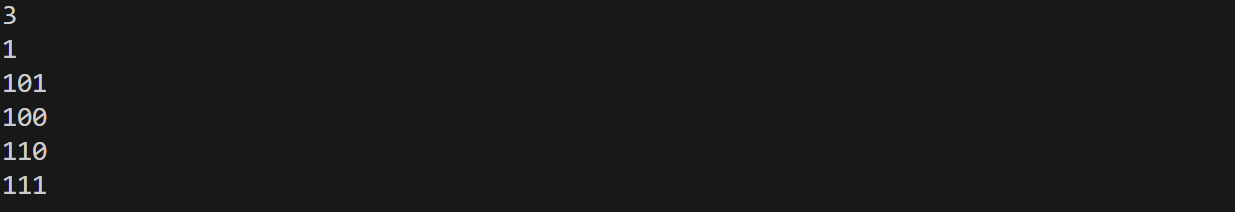
\includegraphics[width=0.9\linewidth]{c3.png}
		\caption{n = 3}
	\end{minipage}
	\qquad%让图片换行,
	\begin{minipage}{0.6\linewidth}
		\centering
		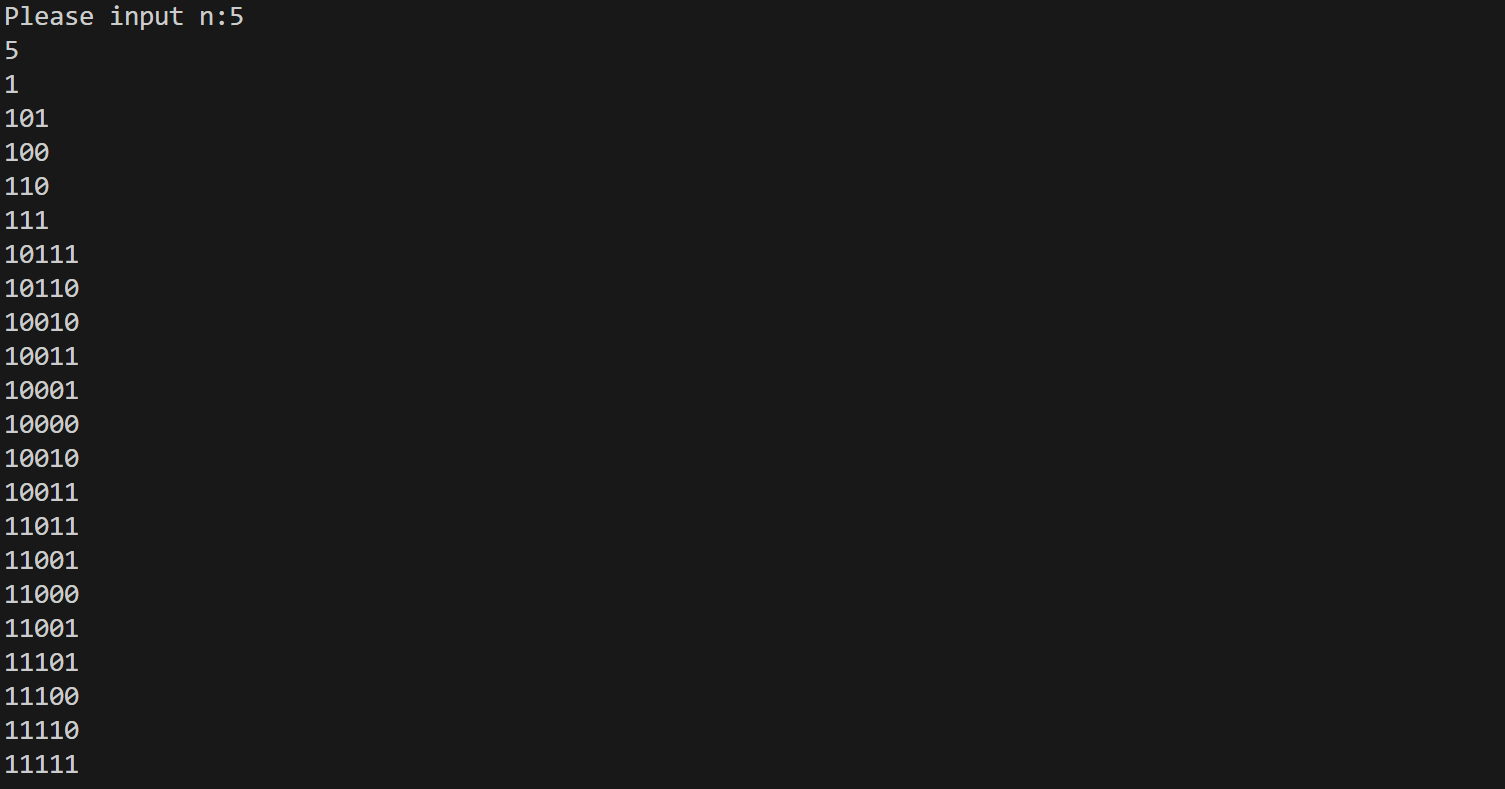
\includegraphics[width=0.9\linewidth]{c5.png}
		\caption{n = 5}
	\end{minipage}
\end{figure*}

上述结果正确,说明思路正确,然后可以转换为汇编语言。

\subsection{流程图}

先画出流程图如下:

\begin{figure*}[htbp]
	\centering
	\begin{minipage}{0.6\linewidth}
		\centering
		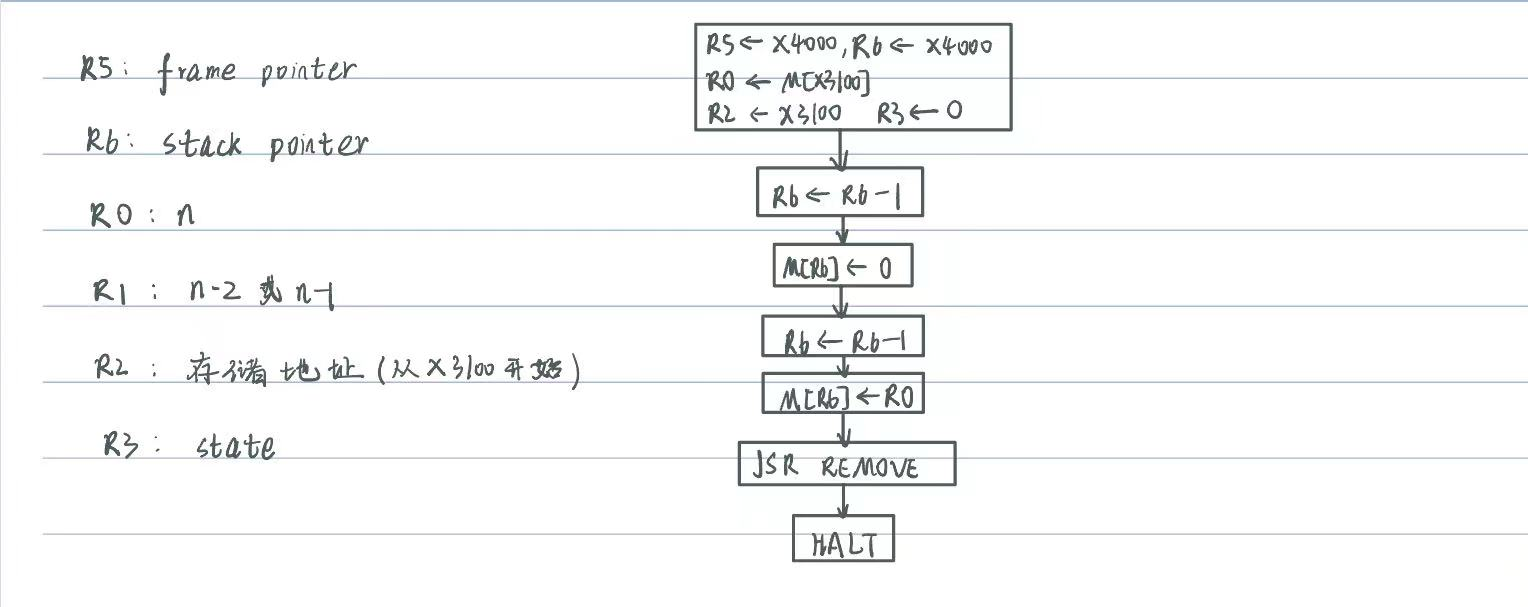
\includegraphics[width=0.9\linewidth]{main.jpg}
		\caption{main}
	\end{minipage}
\end{figure*}
\begin{figure}[htbp]
	\centering
	\begin{minipage}{0.49\linewidth}
		\centering
		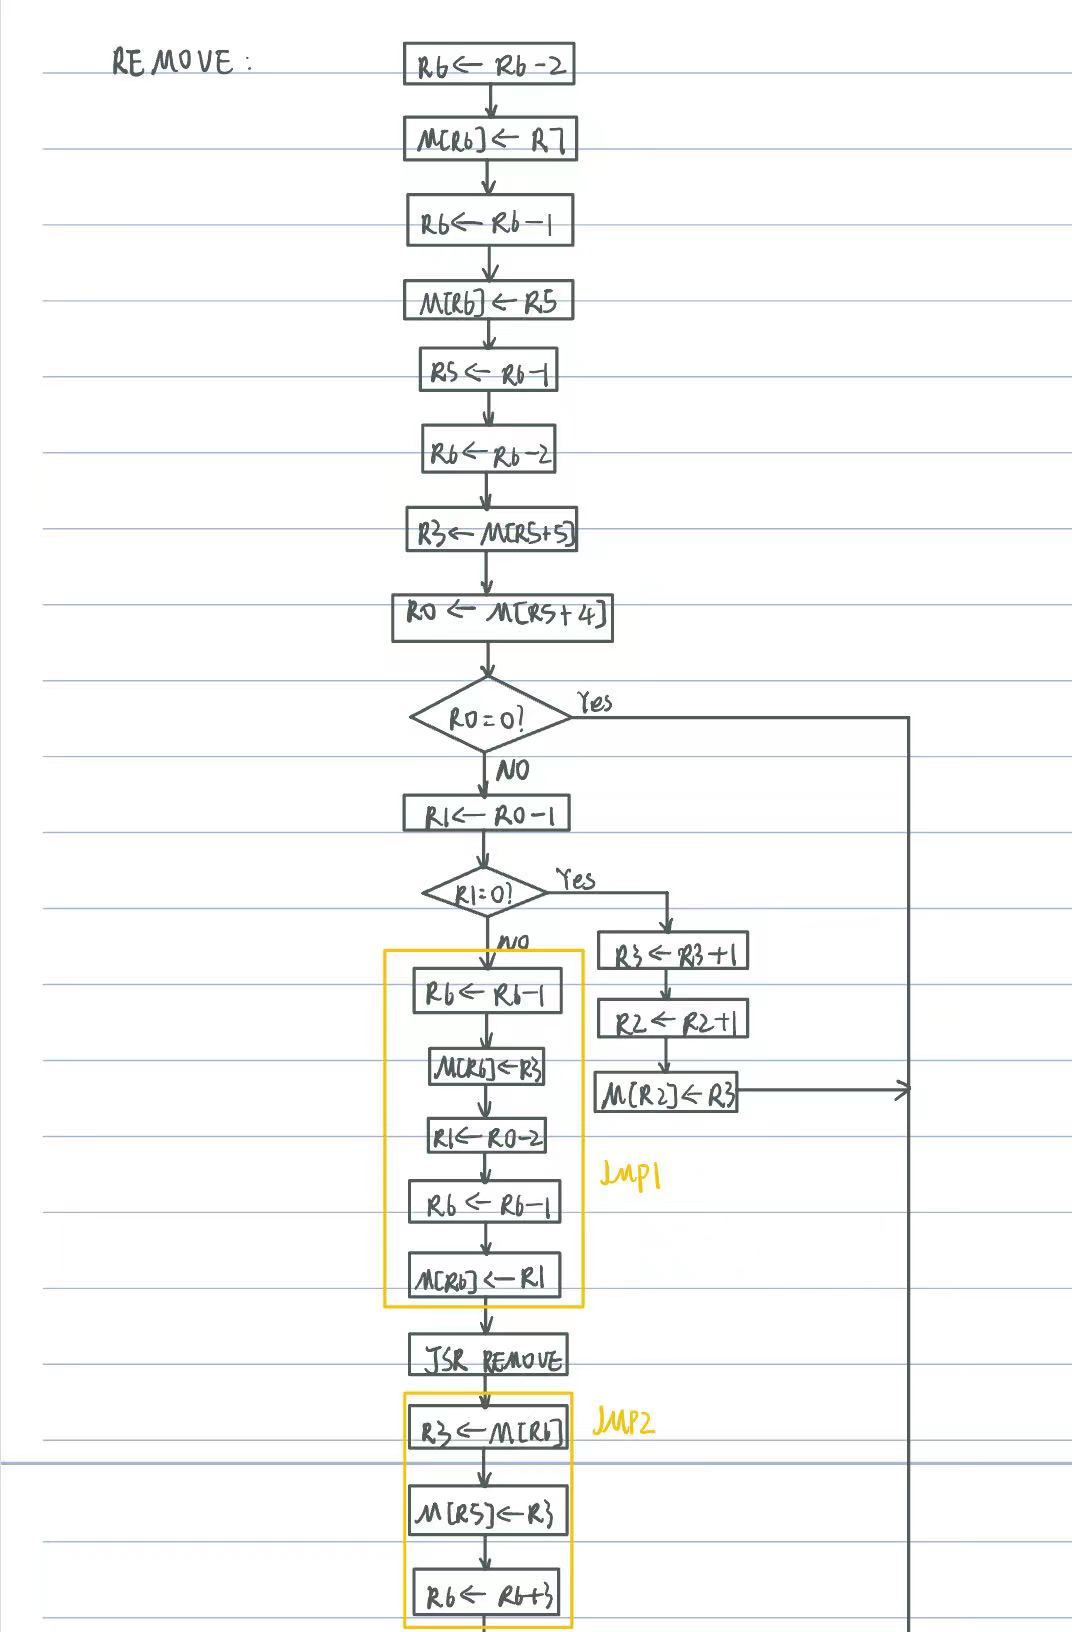
\includegraphics[width=0.9\linewidth]{remove1.jpg}
		\caption{remove}
		%\label{chutian1}%文中引用该图片代号
	\end{minipage}
	%\qquad
	\begin{minipage}{0.49\linewidth}
		\centering
		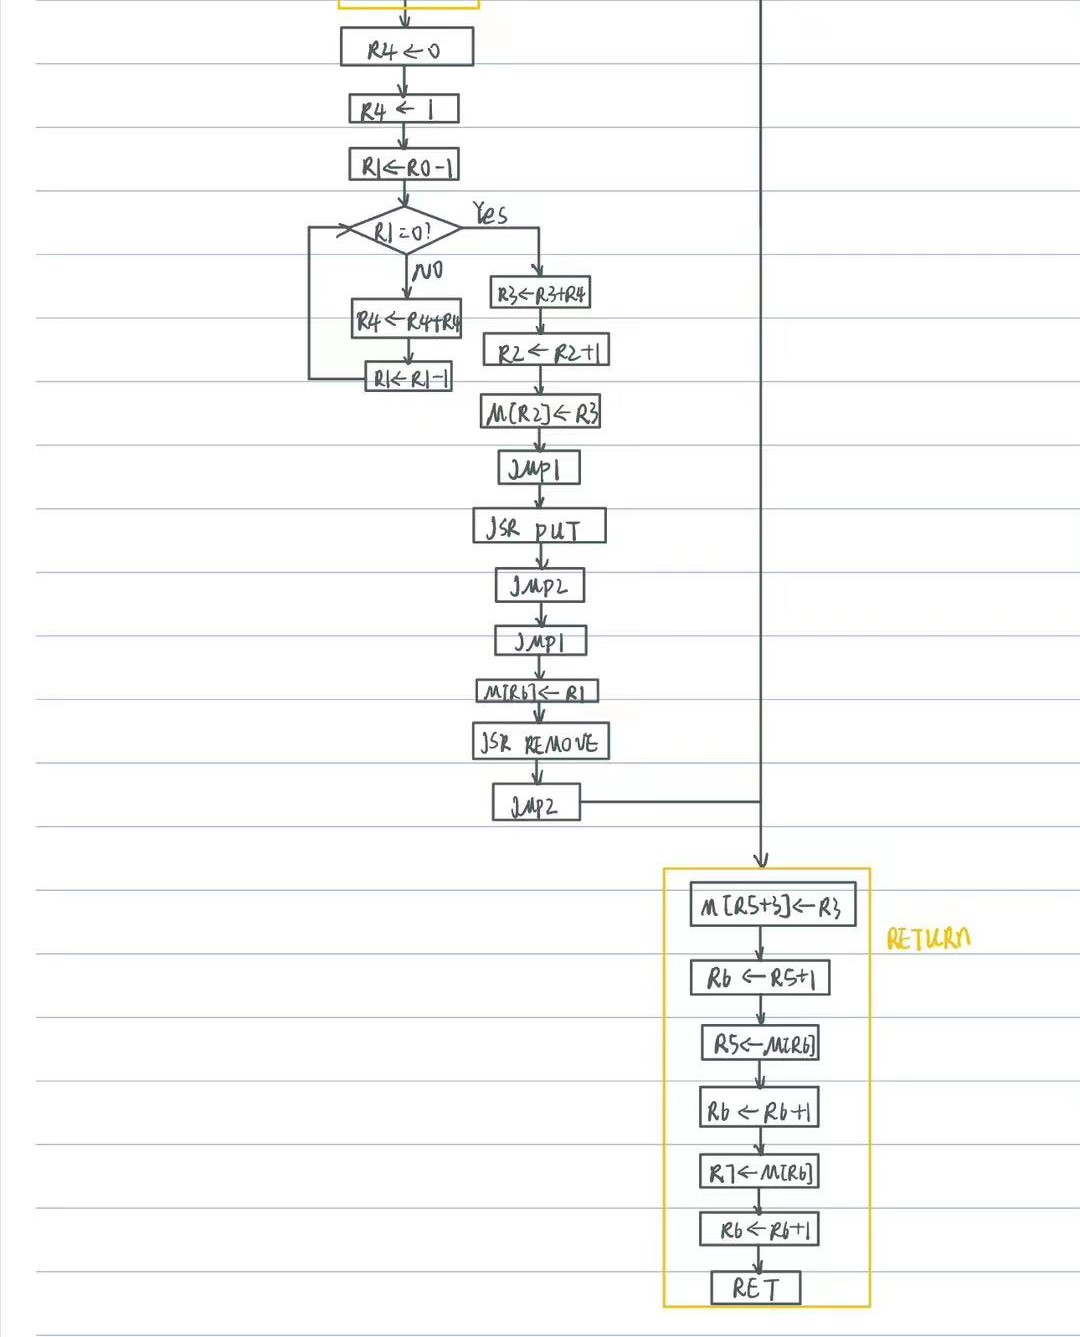
\includegraphics[width=0.9\linewidth]{remove2.jpg}
		\caption{remove(续)}
		%\label{chutian2}%文中引用该图片代号
	\end{minipage}
\end{figure}

由于{\bfseries PUT}的操作与{\bfseries REMOVE}的操作几乎一样,只有极少部分需要更改,所以就没有再画相应的流程图。

\subsection{汇编语言实现}
根据流程图,可以写出汇编代码如下:
\begin{lstlisting}
;
;本题的关键在于使用栈来构造递归子程序REMOVE和PUT
;
            .ORIG   x3000
            LD      R5, BOTTOM          ;R5为frame pointer,初始化为x4000
            LD      R6, BOTTOM          ;R6为stack pointer,初始化为x4000
            LD      R2, START           ;R2为存储state的地址,初始化为x3100
            LDR     R0, R2, #0          ;R0存储n的值
            AND     R3, R3, #0          ;R3用于存储state

            ADD     R6, R6, #-1         ;
            STR     R3, R6, #0          ;state = 0入栈
            ADD     R6, R6, #-1         ;
            STR     R0, R6, #0          ;n入栈
            JSR     REMOVE              ;调用REMOVE子程序
            BRnzp   OVER                ;调用完毕后程序结束,不需要处理返回值
            
            
REMOVE      ADD     R6, R6, #-2         ;为返回值预留空间
            STR     R7, R6, #0          ;保存返回地址
            ADD     R6, R6, #-1         ;
            STR     R5, R6, #0          ;保存caller's frame pointer
            ADD     R5, R6, #-1         ;
            ADD     R6, R6, #-2         ;为局部变量state和n分配空间
            
            LDR     R3, R5, #5          ;R3存储state
            LDR     R0, R5, #4          ;R0存储n
            STR     R3, R5, #0          ;存储局部变量state
            STR     R0, R6, #0          ;存储局部变量n
            BRz     RETURN1             
            ADD     R1, R0, #-1         
            BRz     STORE1              ;n=1时单独处理
            JSR     JMP1                ;做子程序调用前的准备
            JSR     REMOVE              ;递归调用,REMOVE(n-2,state)
            JSR     JMP2                ;做子程序调用后的处理
            AND     R4, R4, #0
            ADD     R4, R4, #1          ;R4 <- 1
            ADD     R1, R0, #-1
JUDGE1      BRnp    LOOP1               ;令R4的第n位为1,后面全为0
            ADD     R3, R3, R4          ;令R3的第n位为1
            ADD     R2, R2, #1          ;存储地址加1
            STR     R3, R2, #0          ;存储state
            JSR     JMP1
            JSR     PUT                 ;PUT(n-2,state)
            JSR     JMP2
            JSR     JMP1
            ADD     R1, R1, #1          ;JMP1中令R1 <- R0-2, 这里需要令R1 <- R0-1, 故还需加1
            STR     R1, R6, #0
            JSR     REMOVE              ;REMOVE(n-1,state)
            JSR     JMP2                ;JMP1中令R1 <- R0-2, 这里需要令R1 <- R0-1, 故还需加1
            BRnzp   RETURN1
                       
            
PUT         ADD     R6, R6, #-2         ;为返回值预留空间
            STR     R7, R6, #0          ;保存返回地址
            ADD     R6, R6, #-1         ;
            STR     R5, R6, #0          ;保存caller's frame pointer
            ADD     R5, R6, #-1         ;
            ADD     R6, R6, #-2         ;为局部变量state和n分配空间
            
            LDR     R3, R5, #5          ;R3存储state
            LDR     R0, R5, #4          ;R0存储n
            STR     R3, R5, #0          ;存储局部变量state
            STR     R0, R6, #0          ;存储局部变量n
            BRz     RETURN1             
            ADD     R1, R0, #-1         ;n=1时单独处理,将最后一位由1变成0
            BRz     STORE2
            JSR     JMP1                ;做子程序调用前的准备
            JSR     PUT                 ;PUT(n-2,state)
            JSR     JMP2
            AND     R4, R4, #0
            ADD     R4, R4, #1
            ADD     R1, R0, #-1
JUDGE2      BRnp    LOOP2               ;R4的第n位为1,后面全为0
            NOT     R4, R4
            ADD     R4, R4, #1          ;将R4取反加1
            ADD     R3, R3, R4          ;将R3的第n位由1变成0
            ADD     R2, R2, #1
            STR     R3, R2, #0
            JSR     JMP1
            JSR     REMOVE              ;REMOVE(n-2,state)
            JSR     JMP2
            JSR     JMP1
            ADD     R1, R1, #1          ;JMP1中令R1 <- R0-2, 这里需要令R1 <- R0-1, 故还需加1
            STR     R1, R6, #0
            JSR     PUT                 ;PUT(n-1,state)
            JSR     JMP2
            BRnzp   RETURN1 
               
            
LOOP1       ADD     R4, R4, R4
            ADD     R1, R1, #-1
            BRnzp   JUDGE1
            
LOOP2       ADD     R4, R4, R4
            ADD     R1, R1, #-1
            BRnzp   JUDGE2
              
            
STORE1      ADD     R3, R3, #1          ;最后一位由0变为1
            ADD     R2, R2, #1          ;存储地址自加1
            STR     R3, R2, #0          ;
            BRnzp   RETURN1             ;
            
STORE2      ADD     R3, R3, #-1         ;最后一位由1变为0
            ADD     R2, R2, #1          ;存储地址自加1
            STR     R3, R2, #0          ;
            BRnzp   RETURN1             ;
            
            
RETURN1     STR     R3, R5, #3
            ADD     R6, R5, #1
            LDR     R5, R6, #0
            ADD     R6, R6, #1
            LDR     R7, R6, #0
            ADD     R6, R6, #1
            RET
            
            
JMP1        ADD     R6, R6, #-1         ;
            STR     R3, R6, #0          ;存储state
            ADD     R1, R0, #-2         ;R1 = n-2
            ADD     R6, R6, #-1         ;
            STR     R1, R6, #0          ;存储n-2
            RET
            
JMP2        LDR     R3, R6, #0          ;获得返回值
            STR     R3, R5, #0          ;存储返回值
            LDR     R0, R6, #3
            ADD     R6, R6, #3          ;子程序的返回值和局部变量出栈
            RET
            
                
START       .FILL   x3100
BOTTOM      .FILL   x4000

OVER        HALT
            .END
\end{lstlisting}


\section{实验结果}


\end{document}
